\section{Jet quenching}
\label{jets_intro}

The vastly increased production cross sections for very high \pT hard-scattered jets at the LHC
compared to RHIC, combined with the moderate growth of soft particle production forming the ``underlying
event'', opened a new era in studies of jet quenching. The improved signal to background allowed the 
use of standard reconstruction techniques, calibration methods, background subtraction methods and 
jet observables developed and well characerized for studies of \pp collisions. 
Typically jets in LHC heavy-ion collisions have been reconstructed using 
the infrared-safe anti-$k_t$ jet clustering algorithm~\cite{Cacciari:2008gp} with the 
radius parameter $R$ varying from $0.2 < R  < 0.5$.

Early measurements of hadron production at RHIC
clearly showed a large suppression (up to a factor of five to six) in the production rates of 
high \pT particles in heavy-ion collisions compared to a properly scaled pp reference distribution. 
\cite{Adcox:2001jp,Adler:2002xw}. Similarly, the ``jet quenching'' phenomenon was observed 
in the suppression of back-to-back hadron production
in more central heavy ion collisions~\cite{Adler:2002xw}. 
\cite{Adcox:2001jp,Adler:2002xw}. Yet nearly a decade after the first observation, a detailed 
understanding of the physics of parton energy loss in the hot and dence medium remained
elusive. Reviews of the theoretical state-of-the art before LHC startup can be 
found in ~\cite{Wiedemann:2009sh,Majumder:2010qh}.

Compared to hadron-based observables such as those employed at RHIC, measurements of reconstructed
jet, dijet and photon-jet final states promise much greater control over the type and kinematics
of the initial scattering process and access to information about the energy flow in the evolution
of the collision process not otherwise accessible. 

\subsection{Dijet correlations}

The first jet-based observables discussed here are derived from dijet correlations. Within hours
after the first heavy-ion collisions at LHC were recorded, it became obvious that there was
a large abundance of events were a high \pT reconstructed jet (e.g. $\pT \approx 100$\GeVc) was
not accompanied by a back-to-back high \pT partner jet.

In the first study of jets in PbPb collisions at LHC used azimuthal correlations and the 
momentum asymmetry between the leading and subleading jets to characterize the modification
of their properties relative to pp collisions \cite{Aad:2010bu}.
The jet pairs were selected to have relative azimuthal angle $\Delta \phi =|\phi_1-\phi_2| > \pi/2$
and their momentum asymmetry was determined as
\begin{equation}
A_J = \frac{E_{T1}-E_{T2}}{E_{T1}+E_{T2}}, \Delta\phi > \frac{\pi}{2}.
\end{equation}
The leading jet was required to have a transverse energy in the calorimeter of $E_{T1} > 100$~GeV,
and the subleading jet was selected to have $E_{T2} > 25$~GeV, after correction for 
the calorimeter energy response. 

In Fig.~\ref{final_4x2} the dijet asymmetry and $\Delta\phi$ distributions for PbPb data (solid markers) 
are shown in four bins of collision centrality. They are compared with PYTHIA MC calculations, including a 
background simulation using the HIJING event generator. Also shown are data from 7\TeV 
\pp collisions (open circles).
\begin{figure}[thb]
\begin{center}
\vspace{-9cm}
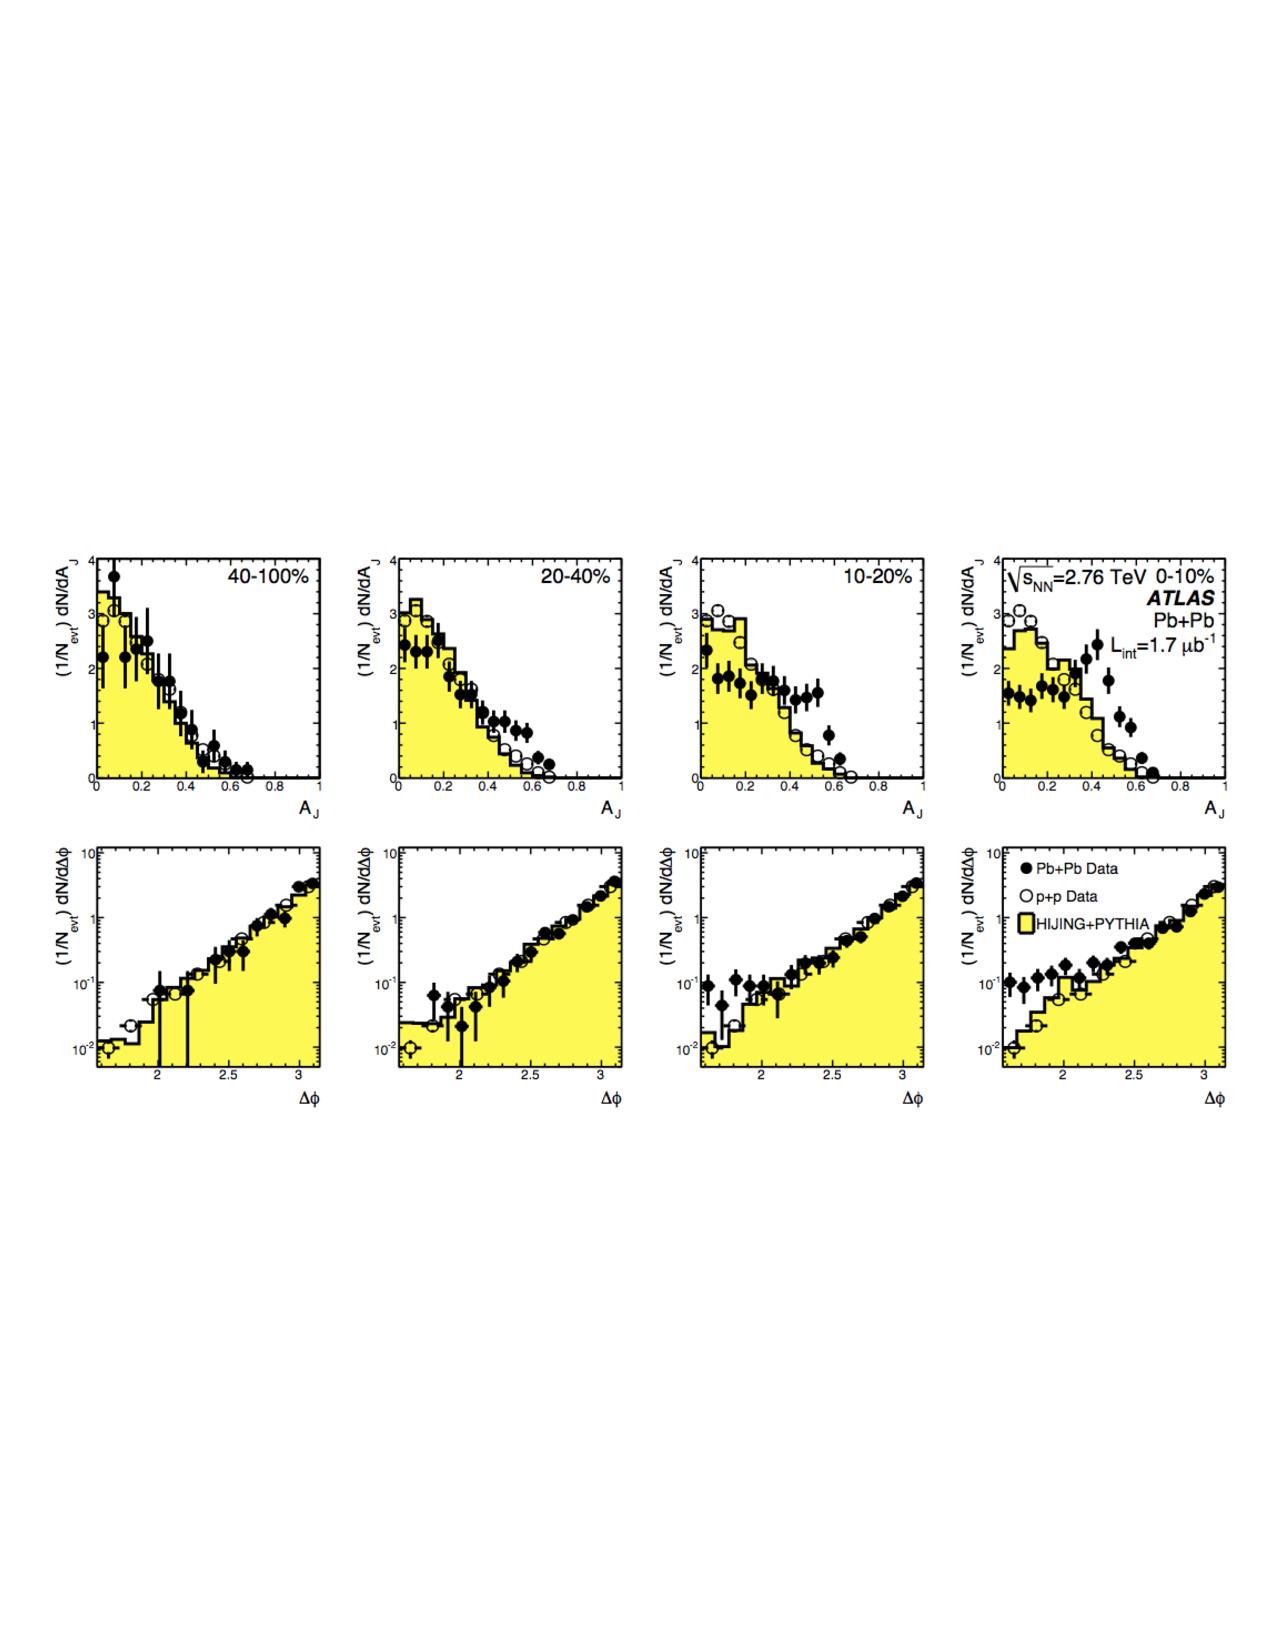
\includegraphics[width=0.9\mboxwidth]{jetfigures/ATLAS_dijet_crop.pdf}
\vspace{-7.5cm}
\caption{
(top) Dijet asymmetry distributions for data (points) and unquenched HIJING with superimposed PYTHIA dijets (solid yellow histograms),
as a function of collision centrality (left to right from peripheral
to central events).  Proton-proton data from $\sqrt{s}=7$ TeV, analyzed with the same jet selection, is shown as open circles.
(bottom) Distribution of $\Delta\phi$, the azimuthal angle between the two jets, for data and HIJING+PYTHIA, also as a function of centrality.
\label{fig:GR:ATLAS_dijet}
}
\end{center}
\end{figure}

A clear centrality evolution of the dijet asymmetry distribution can be seen, while the azimuthal
dijet correlations remain largely unchanged. For peripheral events, the PbPb dijet asymmetry
is comparable to that seen in PYTHIA and \pp collisions. For central events however, 
the $A_J$ distribution widens significantly, showing a large increase in unbalanced
dijet events. The observed trend can be naturally understood in models of parton energy
loss in the hot and dense medium, where the back-to-back partons will typically traverse
different path lengths, and therefore suffer different amounts of energy loss.

The initial ATLAS and CMS dijet asymmetry analyses were extended using a large dataset of PbPb collisions
collected in 2011 by CMS collaboration at $\rootsNN=2.76 TeV$. For this analysis, the events were 
reconstructed using the  CMS ``particle-flow" algorithm~\cite{CMS-PAS-PFT-10-002,MattPFlow}, 
which attempts to identify all stable particles in an
event (electrons, muons, photons, charged and neutral hadrons)
by combining information from all sub-detector systems.
Jets were then reconstructed, after background subtraction, using the anti-$k_T$ sequential recombination algorithm, 
using the {\mbox{FastJet}} framework, with radius parameter R = 0.3~\cite{Cacciari:2008gp}.

To study the momentum dependence of the amount of energy loss,
Fig.~\ref{fig:GR:CMS_dijet_pt} presents the dijet asymmetry in bins of leading jet
\pt, for 0--20\% central events. 
The distributions show the \ptrat\ ratio, instead of $A_j$,  as a more intuitive 
way of quantifying the dijet momentum asymmetry.

\begin{figure}[!h]
\begin{center}
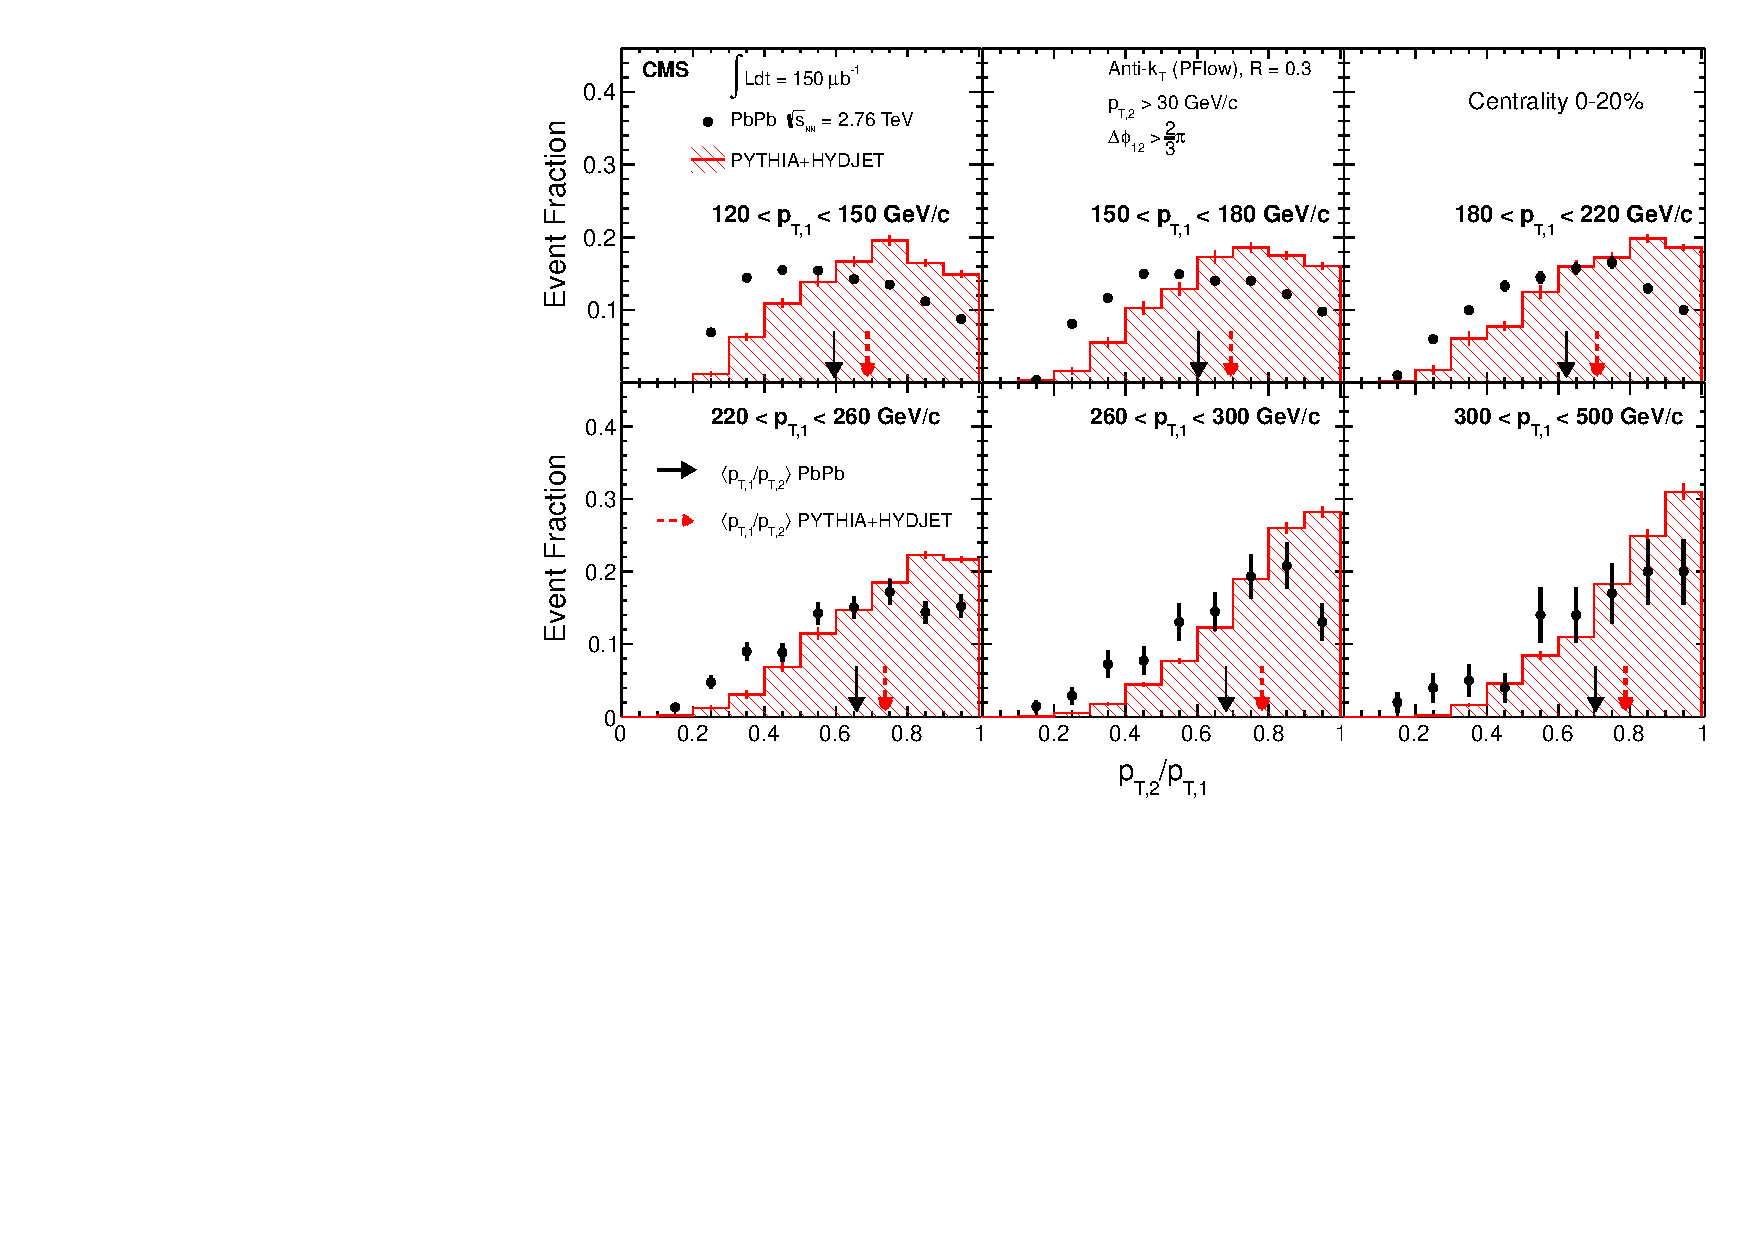
\includegraphics[width=0.49\mboxwidth]{jetfigures/dijet_imbalance5_0to20_pt_20120103_subt.pdf}
\caption{Dijet asymmetry ratio, $A_{J}$, in bins of leading jet transverse momentum from
120 $ < \ptlead < 150$~GeV/c to $\ptlead > 300$~GeV/c for
  subleading jets of $\ptsub> 30$~GeV/c
and $\dphi>2\pi/3$ between leading and subleading jets.
Results for 0--20\% central PbPb events are shown as points, while the histogram
shows the results for
PYTHIA dijets embedded into HYDJET PbPb simulated events. The error bars represent the statistical uncertainties.}
\label{fig:GR:CMS_dijet_pt}
\end{center}
\end{figure}
One observes a strong evolution in the shape of the distribution across the
various \pt\ bins, while a significant difference between PbPb data and 
PYTHYA+HYDJET simulations persists in each \pt\ bin. 
The jet momentum dependence of the energy loss can be examined by measuring the
dijet asymmetry as a function of leading jet momentum. This was studied by CMS,
using $\langle \ptsub/\ptlead \rangle$. Figure~\ref{fig:GR:CMS_pt_ratio} 
shows the \pt dependence of this ratio for three 
bins of collision centrality, with PYTHYA+HYDJET simulations shown 
as squares and PbPb data shown as points. 

\begin{figure}[!h]
\begin{center}
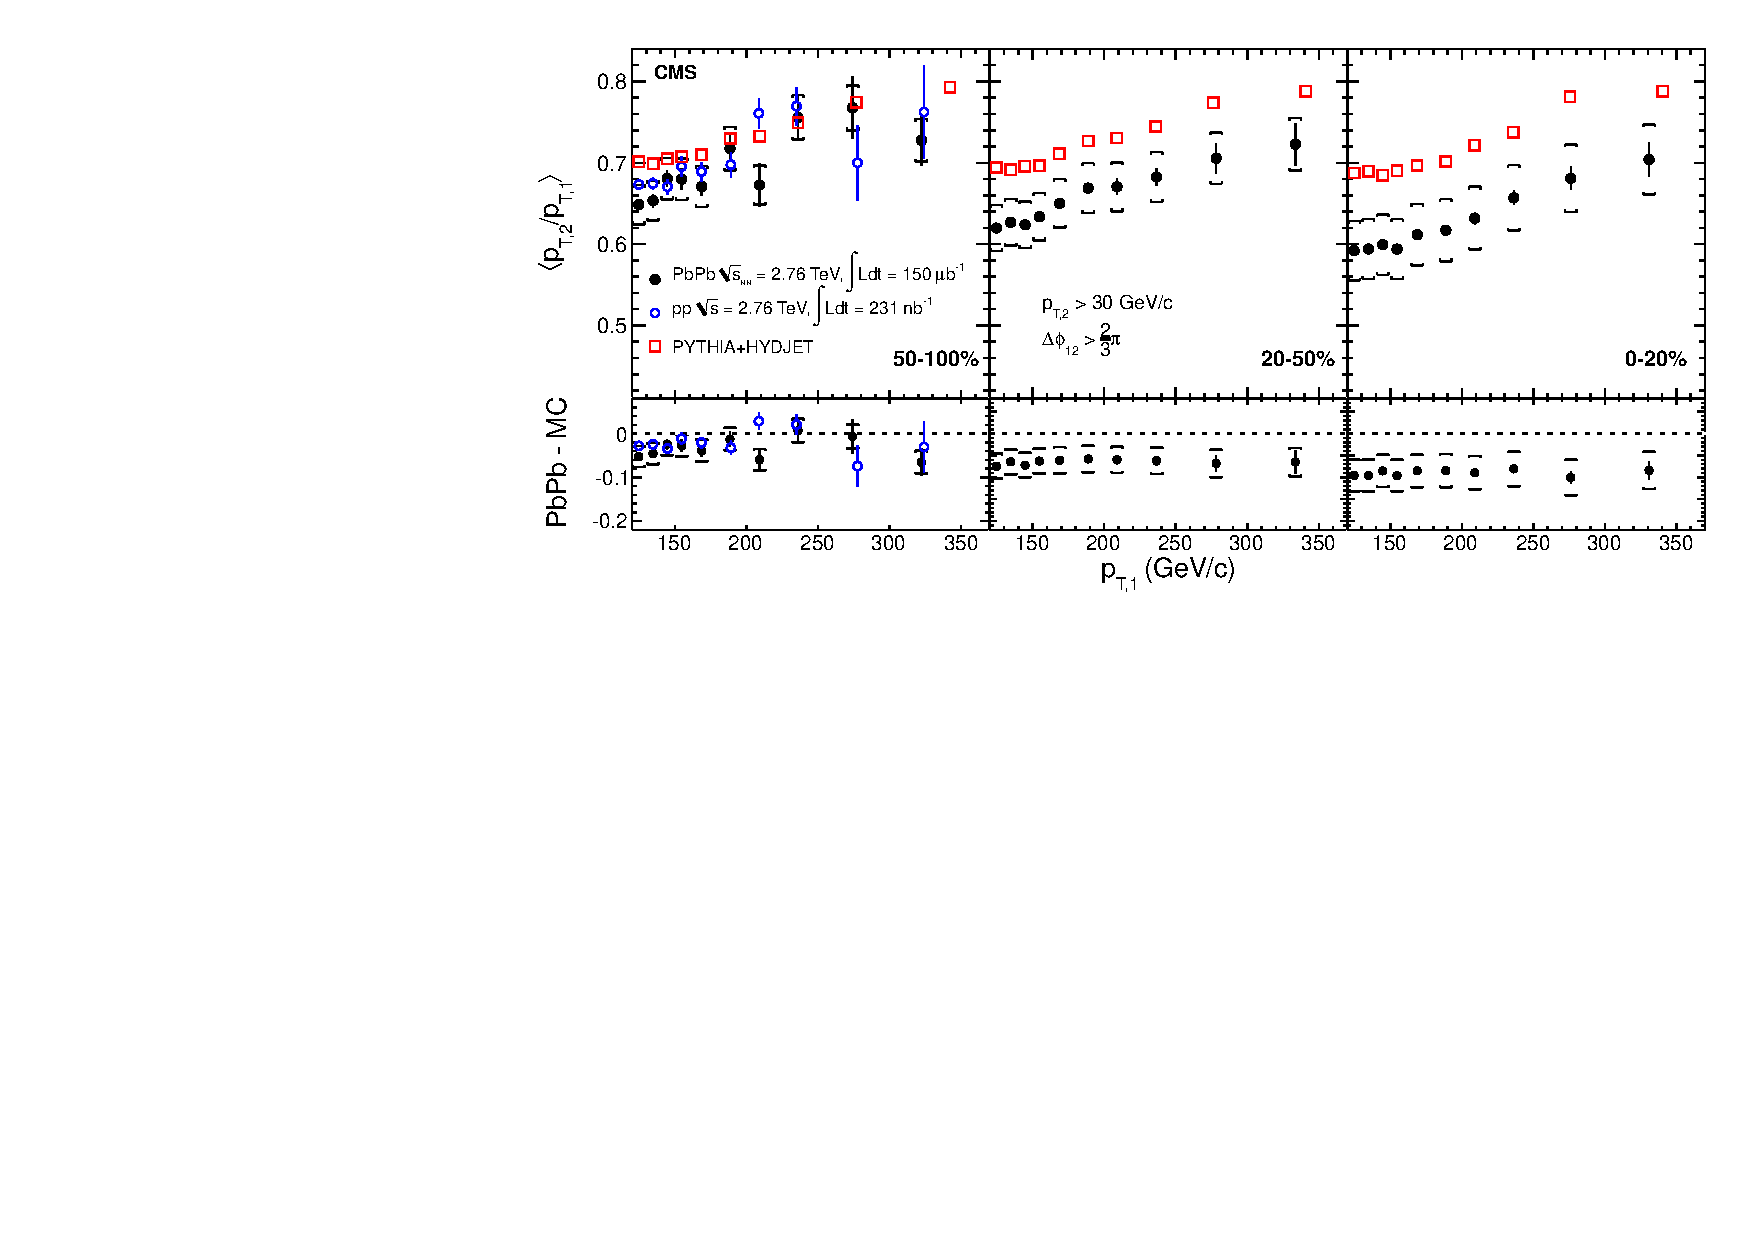
\includegraphics[width=0.49\mboxwidth]{jetfigures/deltaPtOverPt5_lead120_sub30_diff_20120103.pdf}
\caption[]{Average dijet momentum ratio $\ptsub/\ptlead$ as a function of
leading jet \pt for three bins of collision centrality, from peripheral to central collisions,
corresponding to selections of 50--100\%,  30--50\% and 0--20\%  of the total inelastic cross section.
Results for PbPb data are shown as points with vertical bars and brackets indicating
the statistical and systematic uncertainties, respectively.  Results for PYTHIA+HYDJET are shown as squares. In the 50--100\% centrality bin,
results are also compared with pp data, which is shown as the open circles.
The difference between the PbPb measurement and the PYTHIA+HYDJET expectations is shown in the bottom panels. }
\label{fig:GR:CMS_pt_ratio}
\end{center}
\end{figure}

For all data and simulations, a rising trend of $\langle \ptsub/\ptlead \rangle$ as a function
of leading jet momentum is seen. This is a result of the improving jet energy resolution
with increasing jet \pt, and of the evolution in jet kinematics described by the PYTHIA 
simulations. Importantly, the data show a significantly larger jet asymmetry in central events
than in the simulations and in peripheral and \pp data. This effect persists to the 
highest \pt measured, showing that even the highest \pt jets in PbPb collisions ($\pt > 350$\GeVc)
suffer energy loss as they traverse the medium. A detailed understanding of the energy loss
\pt dependence (e.g.\ fractional vs constant energy loss) will require a full jet MC calculation
taking the detector response as a function of \pt into account.

\subsection{Suppression of jet yields}

A complementary approach to the study of parton energy loss using dijet asymmetry measurements
is offered by studies of the nuclear modification factor \Raa of jet yields relative 
to a \pp reference or the centrality evolution of \Rcp relative to peripheral events.

Measurements of the inclusive jet production rates were performed by ATLAS and ALICE.
As a result of the path length dependence of parton energy loss in the medium, 
\cite{Armesto:2011ht} a reduction in the observed jet yield, normalized per 
nucleon-nucleon collision, is expected for more central collisions.

In the ATLAS measurement, the jet suppression was quantified using the central-to-peripheral ratio, 
\Rcp, comparing jet in a given centrality bin to those in the most peripheral bin, after 
normalization to \Ncoll.

\begin{figure}[!h]
\begin{center}
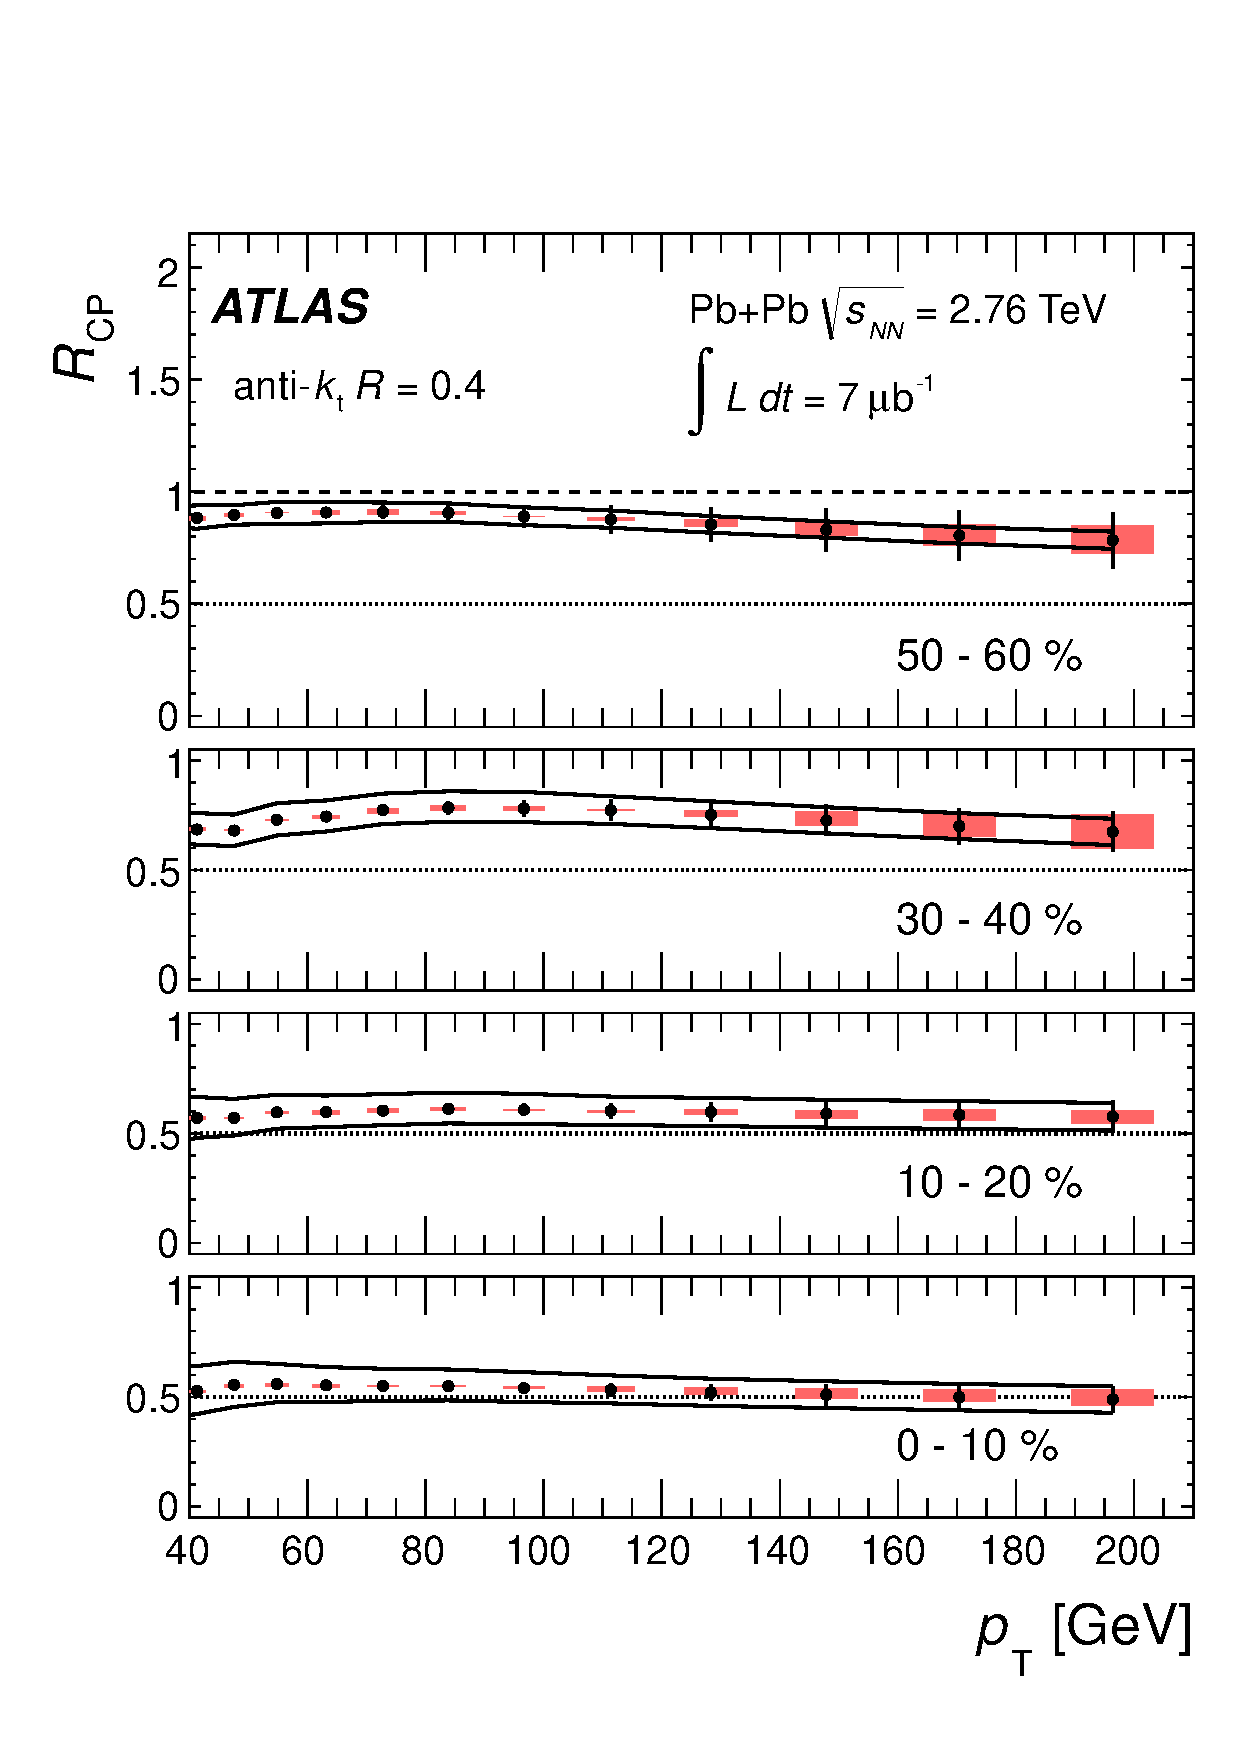
\includegraphics[width=0.49\mboxwidth]{jetfigures/ATLAS_jetRCP_04.pdf}
\caption{
 \Rcp\ values as a function of jet
\pT\ for \RTwo\ (left) and \RFour\ (right) \antikt\ jets
in four bins of collision centrality. The error bars indicate
statistical errors from the unfolding, the shaded boxes indicate
unfolding regularization systematic errors that are partially
correlated between points. The solid lines indicate
systematic errors that are fully correlated between all points.
The horizontal width of the systematic error band is chosen for
presentation purposes only. Dotted lines indicate $\Rcp =
0.5$, and the dashed lines on the top panels indicate $\Rcp = 1$.
}
\label{fig:GR:ATLAS_jet_rcp}
\end{center}
\end{figure}
The resulting \Rcp\ values are shown in Figure~\ref{fig:rcprfour} 
for  \RFour\ jets as a function of jet \pT\ in four bins
of collision centrality.
Uncertainties are shown as statistical uncertainties, partially correlated systematic
uncertainties, and fully correlated uncertainties.

For all centralities only a weak dependence of \Rcp\ on jet \pt is observed. 
In contrast, a strong suppression of the jet yield is evident in
central collisions, with \Rcp\ only reaching a value of about 0.5. 
This is reminiscent of the value of charged hadron \Raa\ observed 
by CMS at very high \pt\, which also reaches a value of about 0.5.
The centrality evolution of \Rcp\ is consistent with expectations
based on the increasing in-medium pathlength traversed by the partons.

Further insight into the pathlenth dependence of parton energy 
loss may be gained by studying the dependence of the jet yield
as a function of azimuthal angle relative to the event plane
in peripheral \PbPb\ collisions. This allows the selection of jets 
traversing different length of the medium at the same medium 
conditions, whereas the centrality dependence of \Rcp\ reflects 
both the changing pathlength and potential changes in the medium
density with centrality.

Related measurements have been performed using the azimuthal dependence 
of charged hadron yields at intermediate \pt 
\cite{Adams:2004wz,Adler:2006bw,Adare:2010sp, ATLAS:2011ah, Abelev:2012di}. 
and very high \pt \cite{Chatrchyan:2012xq}. For mid-peripheral events,
a finite \vtwo for charged hadrons was observed for \pt in excess of 40\GeVc.
Compared to these results, jet based measurements offer the advantage
of a more direct relationship between observed jet \pt\ and the energy
of the initial parton.

\begin{figure}[!h]
\begin{center}
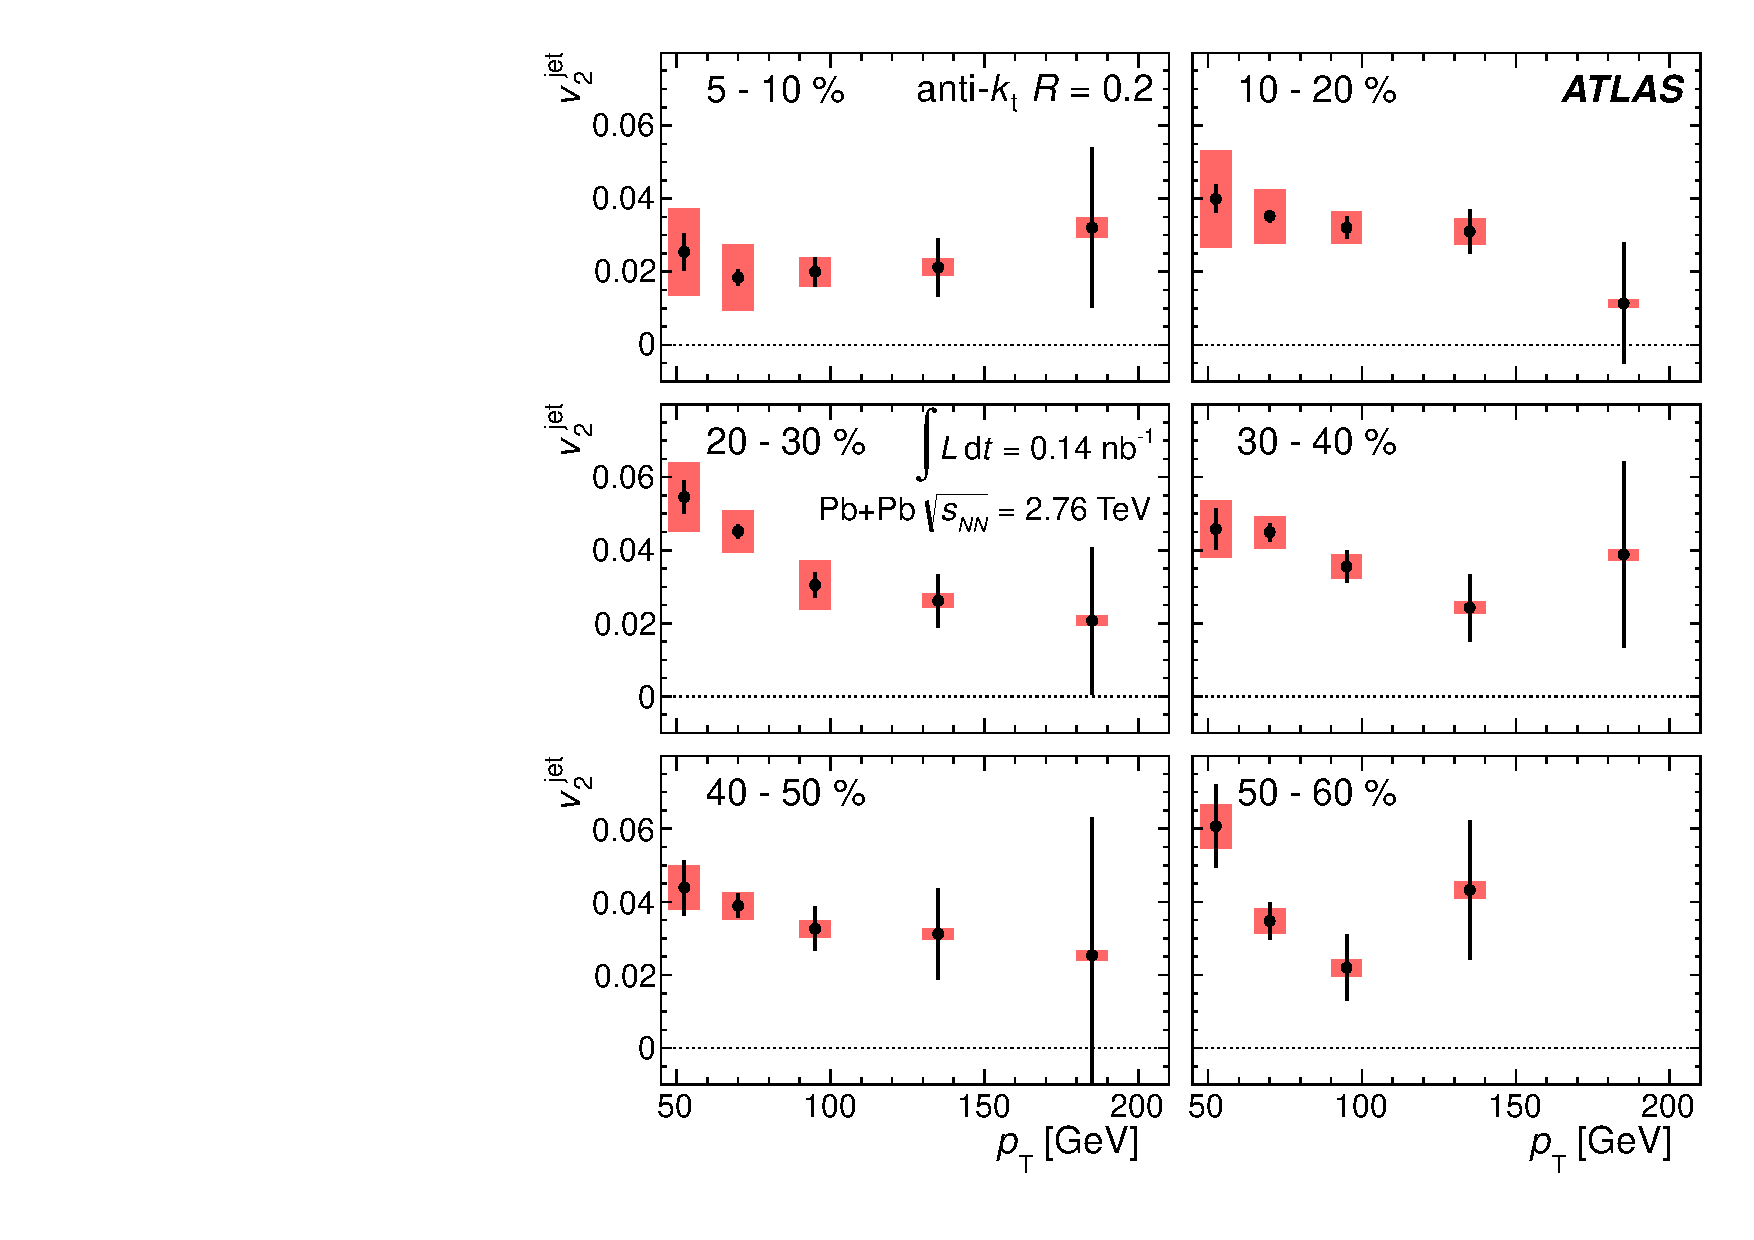
\includegraphics[width=0.49\mboxwidth]{jetfigures/ATLAS_jetv2.pdf}
\caption{\vtjet\ as a function of jet \pTjet\ in each centrality
   interval. The error bars on the points indicate statistical
   uncertainties while the shaded boxes represent the systematic
   uncertainties (see mbox). The horizontal width of the systematic
   error band is chosen for presentation purposes only. }
\label{fig:GR:ATLAS_jet_v2}
\end{center}
\end{figure}

The result of the \vtwo measurement for jets reconstructed with the anti-$k_T$ 
algorithm in 2.76\TeV \PbPb\ collisions is shown in Fig.~\ref{fig:GR:ATLAS_jet_v2}
as a function of jet \pt\ in bins of collision centrality. A finite
value of \vtwo\ is observed for all centrality and \pt, reaching up to 0.05 for
mid-central collisions and low jet \pt. The results are in good agreement
with those for observed for high \pt\ charged hadrons \cite{Chatrchyan:2012xq}.

\subsection{Modification of jet structure}

In addition to the \pt and centrality dependence of the suppresion, its dependence on the 
jet clustering radius parameter is also of great interest, as different energy loss 
mechanisms may lead to different amounts of energy transport out of the jet cone
\cite{Vitev:2008rz, Vitev:2009rd,He:2011pd}. This should manifest as a cone-size 
dependence of the observed jet suppression.
\begin{figure}[!h]
\begin{center}
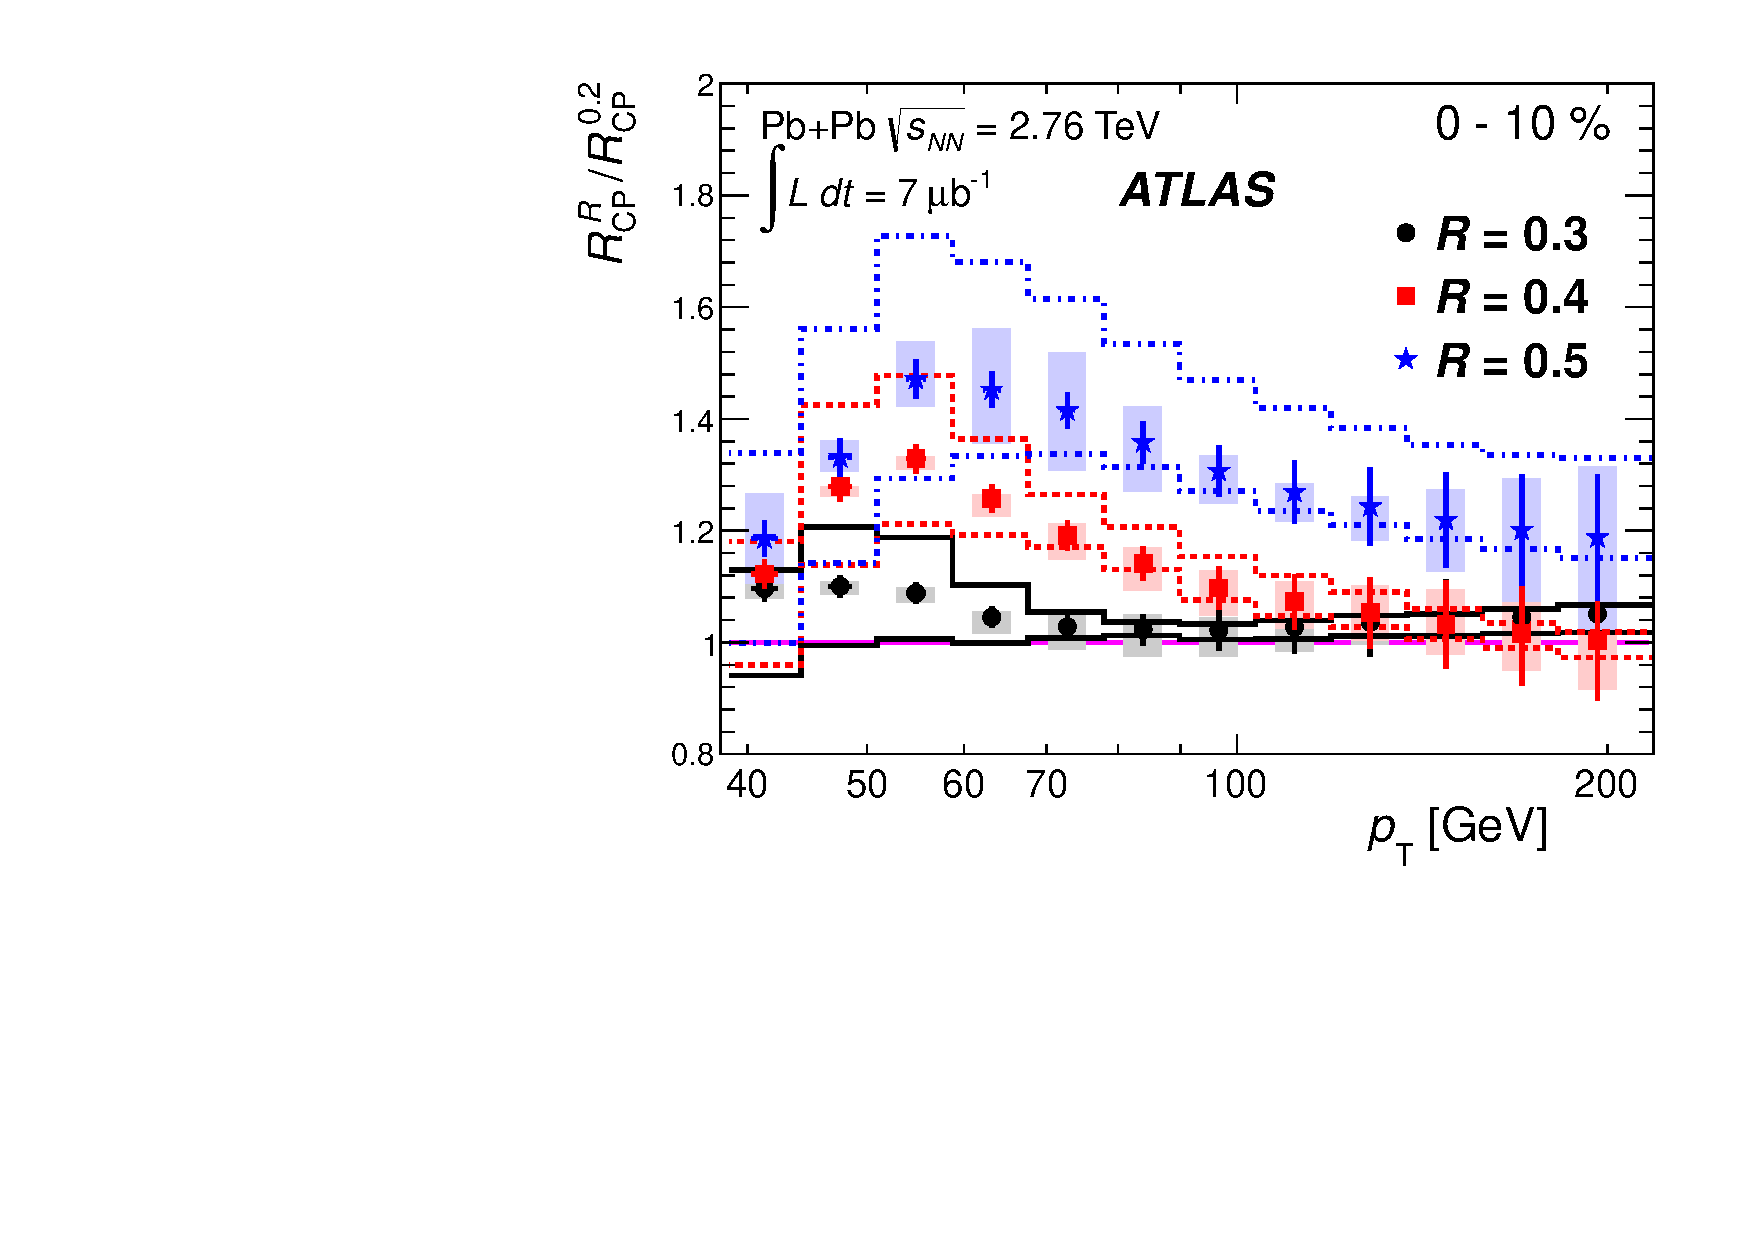
\includegraphics[width=0.49\mboxwidth]{jetfigures/ATLAS_jetRCP_size.pdf}
\caption{
Ratios of \Rcp\ values between $R = 0.3, 0.4$ and 0.5 jets and $R =
0.2$ jets as a function of \pT\ in the 0--10\% centrality bin. The
error bars show statistical uncertainties (see mbox). The shaded boxes
indicate partially correlated systematic errors. The lines indicate
systematic errors that are fully correlated between different \pT\ bins.
}
\label{fig:GR:ATLAS_jetRCP_size}
\end{center}
\end{figure}

Such a dependence can be seen in Fig.\ref{fig:GR:ATLAS_jetRCP_size}, which shows 
shows the ratio of \Rcp\ values for $R = 0.3, 0.4$ and 0.5 jets compared
to an $R = 0.2$ jets baseline as a function of \pt\ for central events.

The cancellation of various systematic uncertainties allows the observation of a 
a significant jet radius dependence of \Rcp, in particular for
lower jet \pt. A detailed comparison needs to consider the \pt\ associated with
using different radius parameters to reconstruct the same jets.

Further insight into modifications of the momentum and angular structure
of jets in heavy-ion collisions can be gained by measurements of 
observables used for jet studies in elementary interactions, such as 
fragmentation functions and jet shapes.
Fragmentation functions described the probability for a parton to fragment into
hadrons carrying certain fractions of the parton energy. 
In vacuum, the parton radiation and splitting processes lead to a
well-understood characteristic shape of the fragmentation function \cite{Dokshitzer:1991wu}.

\begin{figure}[!h]
\begin{center}
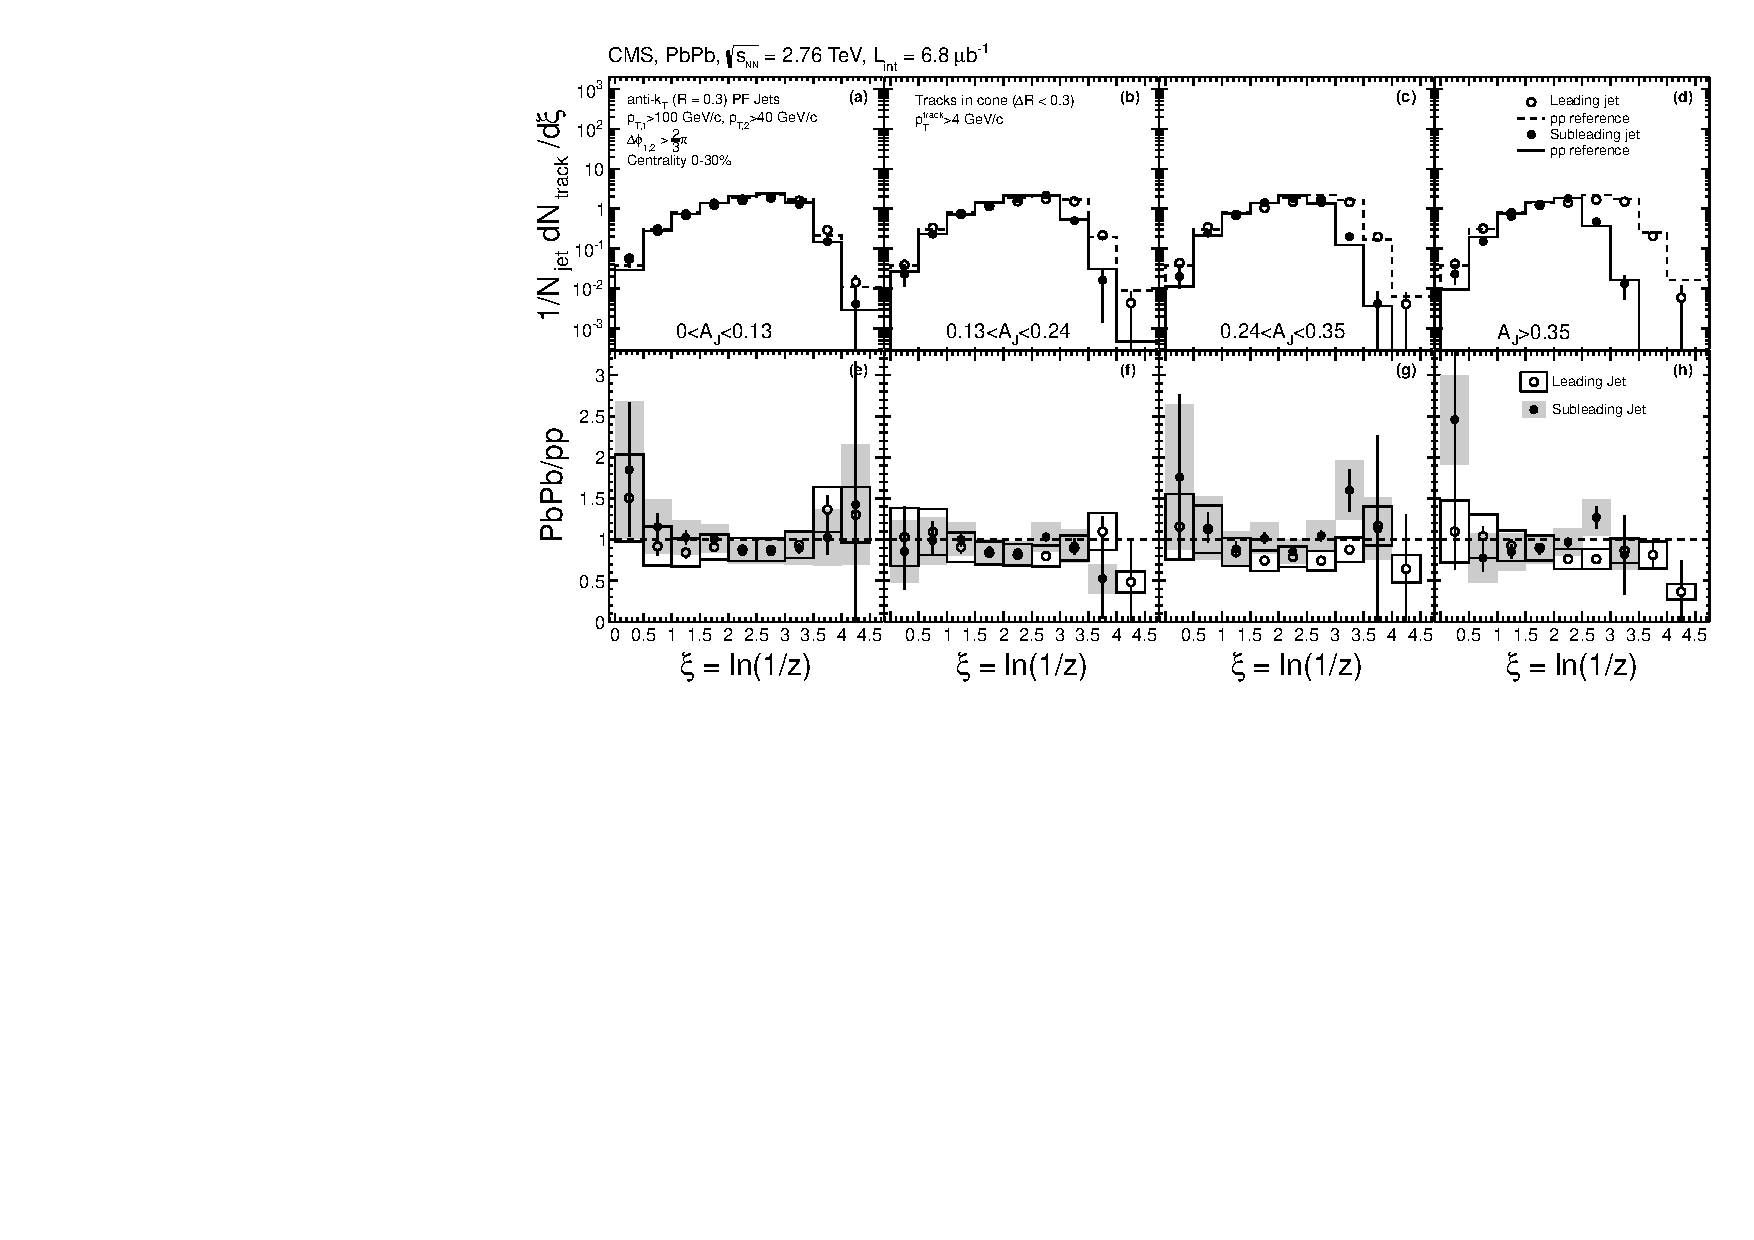
\includegraphics[width=0.98\mboxwidth]{jetfigures/xsi_div_both_effv9_l100s40_0to12_dphi20eta20dr3pt4id1_cwt_ppDiv_gray.pdf}
\caption{(a--d) Fragmentation functions for the leading (open circles) and subleading (solid points) jets in four regions of $\AJ$ in central PbPb collisions compared to the pp reference.
(e--h) Ratio of each fragmentation function to its
pp-based reference.
Error bars shown are statistical. The systematic uncertainty is
represented by hollow boxes (leading jet) or gray boxes (subleading jet).
(i--l) Jet $\pt$ distributions in PbPb collisions in four regions of $\AJ$ (not corrected for efficiency and not unfolded for \pt resolution)
compared to the
pp-based reference
(see mbox). Only statistical uncertainties are shown.
}

\label{fig:GR:CMS_jetFF}
\end{center}
\end{figure}
Figure~\ref{fig:GR:CMS_jetFF} shows the fragmentation functions for
for leading and subleading jets for 0-30\% central collisions. Data for \PbPb\ are shown in 
bins of dijet asymmetry $A_J$, and compared to a \pp\ based reference.
The lower row of plots shows the ratio of the ratios between the PbPb 
and pp-based fragmentation functions.

Within the uncertainties of this first measurement, no significant modification of 
the fragmentation functions in \PbPb\ collisions is observed. This is true even for 
dijets with large asymmetry, i.e.\ where the subleading jet has suffered significant
energy loss. It is important to note however that only hadrons with $\pt > 4$\GeVc
have been considered in this measurement.

Complementary information about the angular structure of the jets and its modification
by the in-medium shower evolution can be obtained by measuring jet shapes, i.e.\ the 
jet transverse momentum profile as a function of radial distance to the jet axis
\cite{MehtarTani:2010ma,Idilbi:2008vm,CasalderreySolana:2011rz,CasalderreySolana:2011rq,Neufeld:2011yh,Blaizot:2012fh,Fickinger:2013xwa}. 
The differential jet shape, $\rho(r)$, is defined as
\begin{equation}
%\rho(r) = \frac{1}{\delta r} \frac{1}{N_{\mbox{jet}}} \sum_\mbox{jets} \frac{\sum\limits_{{r - \delta r/2}}^{{r + \delta r/2}}{\pt^\mbox{track}}}{\pt^\mbox{jet}}
\label{eq:rho(r)}
\end{equation}
Here $r$ is the radial distance from the jet axis
and the transverse momenta of the reconstructed track and jet are 
$\pt^{\mbox{jet}}$ and $\pt^{\mbox{track}}$, respectively.

In the CMS measurement of jet shapes, the jet cone is divided into six concentric rings 
with radial width $\delta r = 0.05$. The transverse momentum profile is determined using
the \pt\ sum for charged particles with $\pt > 1\GeVc$ in each ring, compared to 
the fraction of the total jet \pt carried by these particles. As for the fragmentation
functions, the \PbPb\ jet shapes are compared to a \pp\ based reference.

\begin{figure}[!h]
\begin{center}
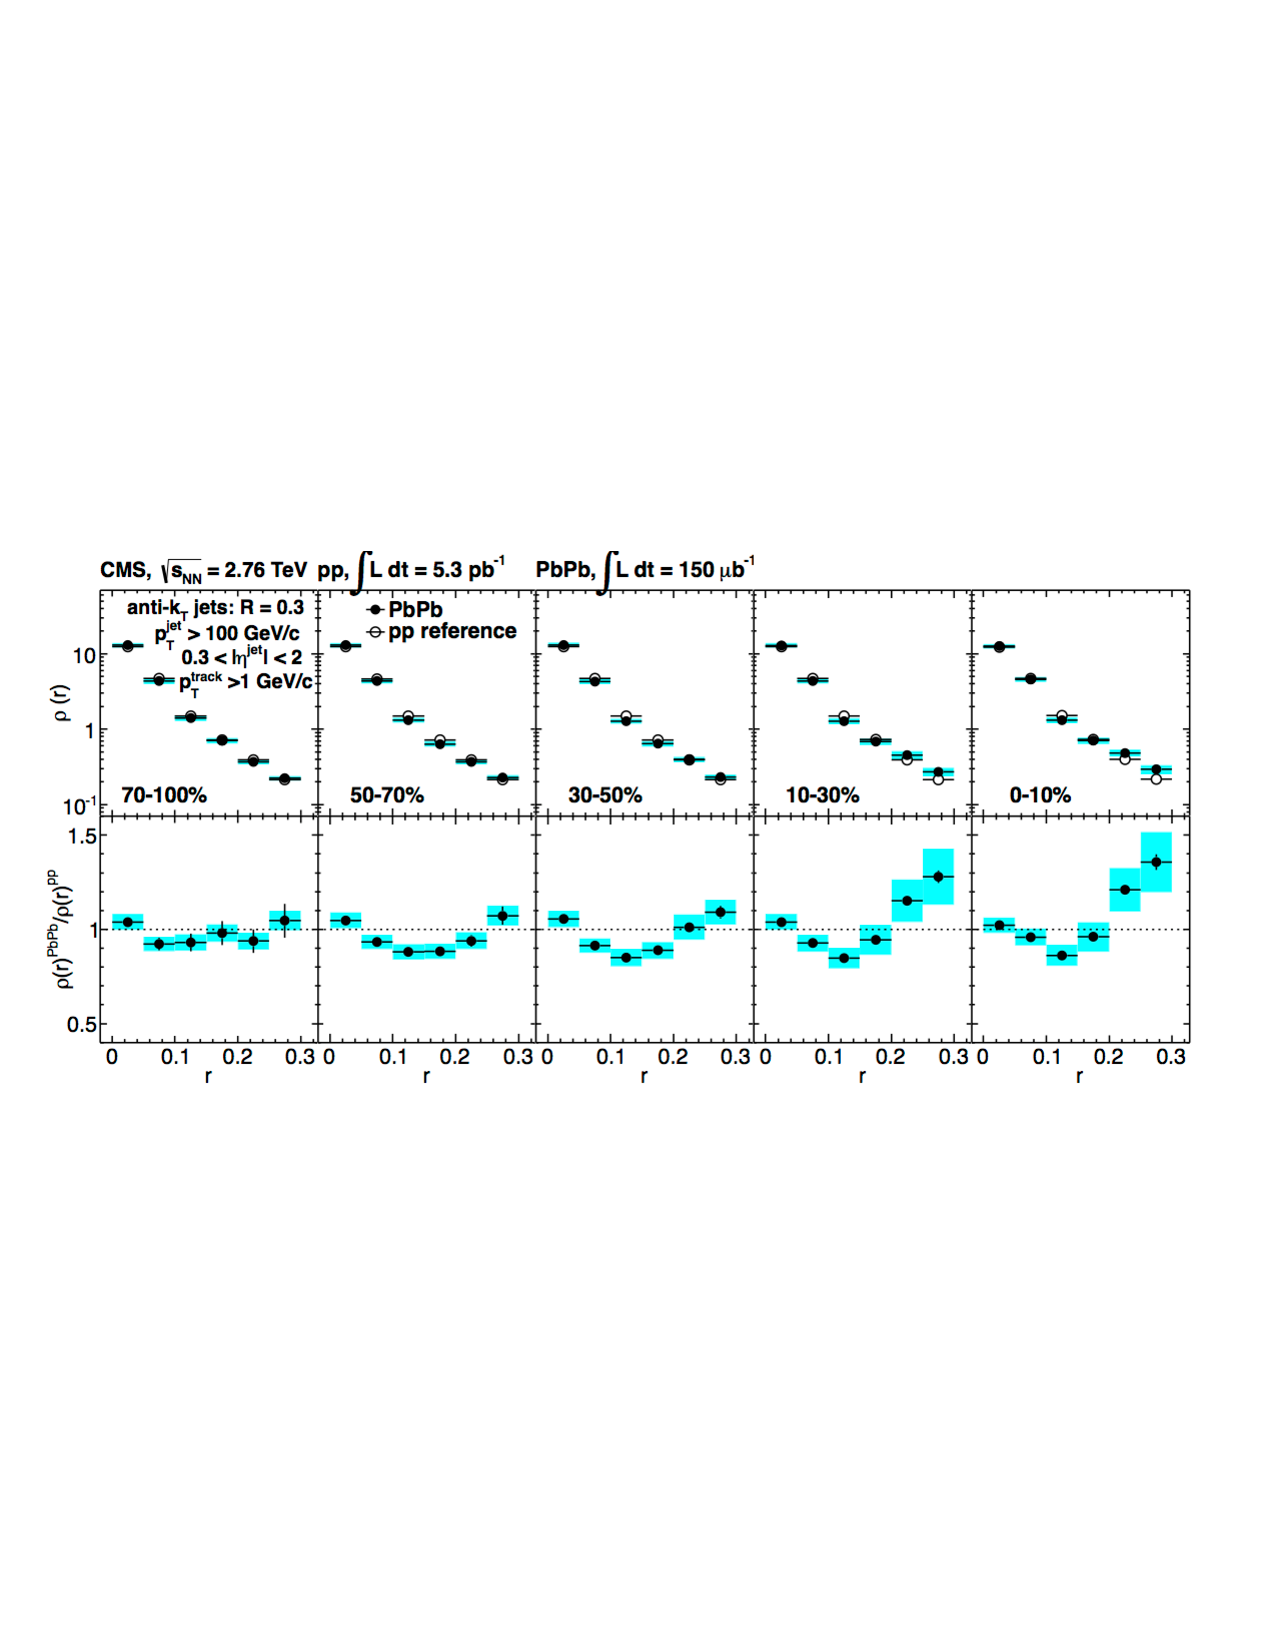
\includegraphics[width=0.98\mboxwidth]{jetfigures/JetShapes_GR.pdf}
\caption{\label{fig:JSRatio}
(Color online) Top row: Differential jet shapes in \PbPb collisions (filled circles)
 as a function of distance from the jet axis for inclusive jets with $\pt^{\mbox{jet}} >100\GeVc$ 
and $0.3 < |\eta| < 2$ in
five \PbPb centrality intervals. The measurements use charged particles with  $\pt^{\mbox{track}} > 1\GeVc$.
The \pp-based reference shapes  are shown with open symbols.
The shaded regions represent the systematic uncertainties for the measurement performed in \PbPb collisions, with the
statistical uncertainties too small to be visible.
Bottom row: Jet shape nuclear modification factors, $\rho(r)^{\PbPb}/\rho(r)^{\pp}$.
The error bars show the statistical uncertainties, and the shaded boxes indicate the systematic uncertainties. }
\label{fig:GR:CMS_jetshapes}
\end{center}
\end{figure}

The top row of Fig.~\ref{fig:GR:CMS_jetshapes} shows the differential jet shapes measured in \PbPb\ 
collisions and the \pp\ based reference, while the bottom row shows the ratio of the \PbPb\ and \pp\ 
distributions. The results are presented in five bins of collision centrality, from
most peripheral 70--100\% (left) to most central 0--10\% (right). For 
both systems, only a small amount of the total jet energy 
is carried by particles more than  $r> 0.2$ away from the jet axis. However, for central 
\PbPb\ collisions a large enhancement of the energy fraction at the largest distance
to the jet axis ($r = $0.25-0.3) can be seen.
This is qualitatively consisten with the \Rcp\ ratios for different jet radii seen by ATLAS, 
where also an additional part of the jet energy is captured when moving beyond $R = 0.2$, and is 
in line with the trends predicted in \cite{Vitev,Renk:2009hv}, although these calculations were
done for a different energy and at parton level, rather than after jet clustering.

\subsection{Energy flow in dijet events}

The requirements of the background subtraction procedure limit the track-jet correlation study
to tracks with $p_{\mathrm{T}} > 1.0$~\GeVc\  and $\Delta R < 0.8$. Complementary information about the
overall momentum balance in the dijet events can be obtained using the projection of missing
\pt\ of reconstructed charged tracks onto the leading jet axis. For each event, this
projection was calculated as

\begin{equation}
\displaystyle{\not} p_{\mathrm{T}}^{\parallel} =
\sum_{\rm i}{ -p_{\mathrm{T}}^{\rm i}\cos{(\phi_{\rm i}-\phi_{\rm Leading\ Jet})}},
\end{equation}
where the sum is over all tracks with $\pt > 0.5$~\GeVc\ and $|\eta| < 2.4$. The results were
then averaged over events to obtain $\langle \displaystyle{\not} p_{\mathrm{T}}^{\parallel} \rangle$.
No background subtraction was applied, which allows this study to include the $|\eta_{jet}| < 0.8$ and 
$0.5 < p_{\mathrm{T}}^{\rm Track} < 1.0$~\GeVc\ regions not accessible for the study in Section~\ref{sec:track_jet_correlations}.
The leading and subleading jets were again required to have $|\eta| < 1.6$.

In Fig.~\ref{fig:MissingpT}, $\langle \displaystyle{\not} p_{\mathrm{T}}^{\parallel} \rangle$
is shown as a function of \AJ\ for two centrality bins, 30--100\% (left) and 0--30\% (right).
Results for {\sc{pythia+hydjet}} are presented in the top row, while the bottom row shows the results
for \PbPb\ data.
Using tracks with $|\eta| < 2.4$ and $\pt > 0.5$~\GeVc, one sees
that indeed the momentum balance of the events, shown as solid circles, is recovered within uncertainties,
for both centrality ranges and even for events with large observed dijet asymmetry, in both data and simulation.

\begin{figure}[!h]
\begin{center}
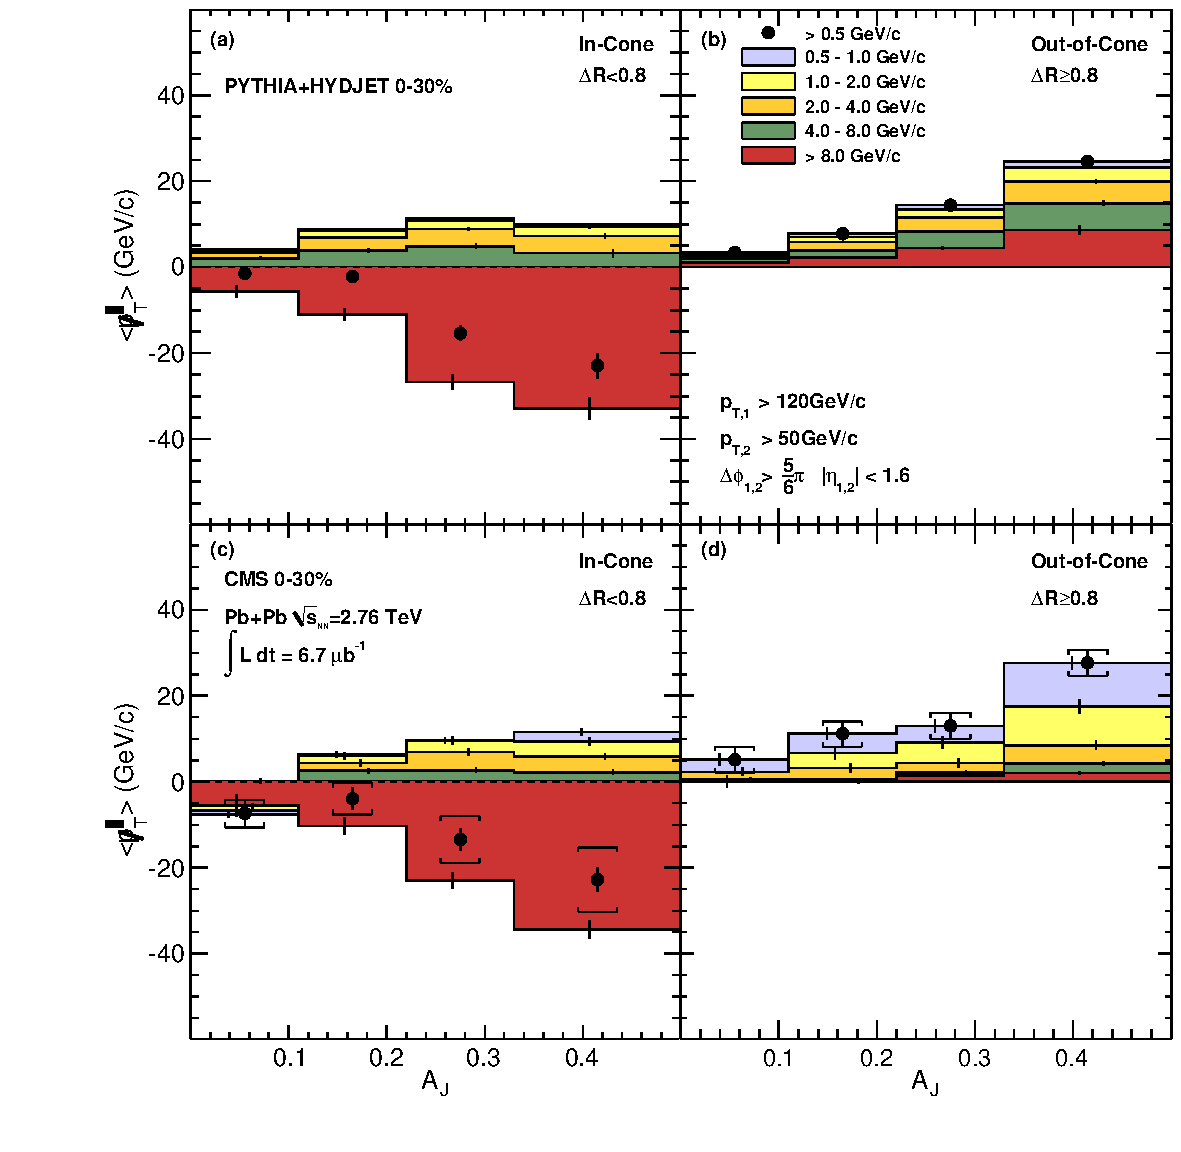
\includegraphics[width=0.98\mboxwidth]{jetfigures/missingPtParallel-Corrected-data-InConeOutConeDPhiCut_ntv6_2.pdf}
\caption{Average missing transverse momentum,
$\langle \displaystyle{\not} p_{\mathrm{T}}^{\parallel} \rangle$,
for tracks with $\pt > 0.5$\GeVc, projected onto the leading jet axis (solid circles).
The $\langle \displaystyle{\not} p_{\mathrm{T}}^{\parallel} \rangle$ values are shown as a function of dijet asymmetry
$A_J$ for 0--30\% centrality, inside ($\Delta R < 0.8$) one of the leading or subleading jet cones (left) and
outside ($\Delta R > 0.8$) the leading and subleading jet cones (right).
For the solid circles, vertical bars and brackets represent
the statistical and systematic uncertainties, respectively.
For the individual $\pt$ ranges, the statistical uncertainties are shown as vertical bars. }
\label{fig:GR:CMS_missingpT}
\end{center}
\end{figure}

Further insight into the radial dependence of the momentum balance can be gained by studying
$\langle \displaystyle{\not} p_{\mathrm{T}}^{\parallel} \rangle$ separately for tracks inside cones of size $\Delta R = 0.8$
around the leading and subleading jet axes, and for tracks outside of these cones. The results of this study for central events
are shown in Fig.~\ref{fig:MissingpTInConeOutCone} for the in-cone balance and out-of-cone balance for MC and data.
As the underlying \PbPb\ event in both data and MC is not $\phi$-symmetric on an event-by-event basis, the back-to-back requirement
was tightened to $\dphi > 5 \pi/6$ for this study.

One observes that for both data and MC an in-cone imbalance of $\langle \displaystyle{\not} p_{\mathrm{T}}^{\parallel} \rangle \approx
-20$~\GeVc\ is found for the $\AJ > 0.33$ selection. In both cases this is balanced by a corresponding out-of-cone
imbalance of  $\langle \displaystyle{\not} p_{\mathrm{T}}^{\parallel} \rangle \approx 20$~\GeVc. However, in the \PbPb\ data
the out-of-cone contribution is carried almost entirely  by tracks with $0.5 < \pt < 4$~\GeVc\, whereas in MC more than 50\% of the balance
is carried by tracks with $\pt > 4$~\GeVc, with a negligible contribution from $\pt < 1$~\GeVc.


The {\sc{pythia+hydjet}} results are indicative of semi-hard initial or final-state radiation as the underlying cause for large
\AJ\ events in the MC study. This has been confirmed by further studies which showed that in {\sc{pythia}} the momentum balance
in the transverse plane for events with large \AJ\ can be restored if a third jet with $\pt > 20$~\GeVc, which is present in more
than 90\% of these events, is included. This is in contrast to the results for large-\AJ\ \PbPb\ data, which show that a
large part of the momentum balance is carried by soft particles ($\pt < 2$~\GeVc) and radiated
at large angles to the jet axes ($\Delta R > 0.8$).

\subsection{Photon-jet correlations}

In PbPb collisions at the Large Hadron Collider (LHC), the
effects of the produced medium have been studied using back-to-back
dijets which were observed to be significantly unbalanced in their transverse momenta~\cite{Chatrchyan:2011sx,Aad:2010bu,CMS:2012ni}. The advantage of the large yield of dijets (as compared to \photonjet\ pairs)
is, however, offset by a loss of information about the initial properties of the probes, i.e.\
prior to their interactions with the medium.
Correlating two probes that both undergo energy loss also
induces a selection bias towards scatterings occurring at,
and oriented tangential to, the surface of the medium.
At leading order (LO), photons are produced back-to-back with an associated parton (jet) having close
to the same transverse momentum.
Furthermore, these photons do not strongly interact with the medium.
The yields of isolated photons in \PbPb{} collisions were found to match
the expectation based on \pp{} data and the number of nucleon-nucleon
collisions, with a modification factor of $R_{AA} = 0.99\pm
0.31\mbox{(stat.)}\pm 0.26\mbox{(syst.)}$~\cite{HIPhoton}.
Therefore, \photonjet\ production has been hailed as the ``golden channel'' to
investigate energy loss of partons in the medium \cite{Wang:1996yh,Wang:1996pe}.

``Prompt photons'' are photons produced directly in the hard
sub-processes. Experimentally, events with enriched production of prompt photons are
selected using an isolation requirement, namely that the additional energy
in a cone of fixed radius around the direction of the reconstructed
photon be less than a specified value~\cite{HIPhoton}. This restriction
yields ``isolated photons'' ($\gamma$), which consist
mostly of prompt photons produced directly in the initial hard scattering.
Background photons from the decays of neutral mesons, such as $\Pgpz$,
$\Pgh$, and $\omega$, are suppressed by this isolation requirement, as
they are predominantly produced via jet fragmentation.
The goal of this analysis is to characterise possible modifications of jet properties as a function of centrality using isolated-\photonjet\ events in \PbPb\ collisions.
The properties of isolated-\photonjet{} pairs are studied
via the azimuthal angular correlation in $\dphijg = |\phij - \phig|$ and the
transverse momentum ratio given by
$\xjg = \ptj/\ptg$.
Photons with transverse momentum of
$\ptg > 60\GeVc$ are selected in a pseudorapidity range of
$|\eta^\gamma\|<1.44$, using isolation criteria detailed in Sections \ref{sec:MC} and \ref{sec:photon_reco}.
These photons are then correlated with jets having $\ptj > 30\GeVc$
and $|\eta^{\mbox{Jet}}|<1.6$.
Parton energy loss due to induced gluon radiation can lead to a shift of the \xjg\
distribution towards lower values.  In addition, parton energy loss
can cause reconstructed jets to fall below the $\ptj > 30\GeVc$
threshold, leading to a reduction of the fraction of photons with an associated jet.

The asymmetry ratio
$\xjg= \ptj/\ptg$ is used to quantify the \photonjet\ momentum imbalance. In addition to the jet and photon selections used in
the \dphijg\ study, we further impose a strict $\dphijg >
\frac{7}{8}\pi$ cut to suppress contributions from background jets.
Note that \photonjet\ pairs for which the associated jet falls below the $30\GeVc$
threshold are not included in the $\xjg$ calculation. This limits the bulk of the $\xjg$ distribution to 
$\xjg > 0.5$.
Figure~\ref{fig:InclPtRatio_qcdPhoRef_pp2760-xJ30G60} shows the centrality dependence of \xjg\ for
\PbPb collisions as well as that for \PYTHYD{}
simulation where \PYTHIA{} contains inclusive isolated photon
processes. The \avexjg{} obtained from \PYTHIA{} tunes Z2 and D6T
agree to better than 1\%.
Overlaid in the peripheral bin is the \avexjg\ for 2.76~TeV pp data,
showing consistency to the MC reference. However the poor statistics
of the \pp\ data and the 50--100\% \PbPb{} centrality bin do not offer a strong constraint on a specific MC reference.
However, further studies using the 7\TeV high statistics \pp\ data showed a
good agreement in \avexjg{} between data and \PYTHIA{}, justifying the
use of \PYTHYD{} as an un-modified reference.
The dominant source of systematic uncertainty in \avexjg{} is
the relative \photonjet{} energy scale. Its impact on the probability
density of $\xjg$ is approximately 10\%
for the intermediate region of $0.6 < \xjg < 1.2$.
The normalisation to unity causes a point-to-point anticorrelation in the
systematic uncertainties, where the upward movement of the probability
density at small $\xjg$ has to be offset by the corresponding downward movement
at large $\xjg$. This is represented by the
separate open and shaded red systematic uncertainty boxes in Fig.~\ref{fig:InclPtRatio_qcdPhoRef_pp2760-xJ30G60}.
For a given change in the energy scale, all points would move together in the direction
of either the open or shaded red box.
The $\npart$ dependence of the mean value $\avexjg$ is shown in Fig.~\ref{fig:resultsummarybc}(a).

\begin{figure}[!h]
\begin{center}
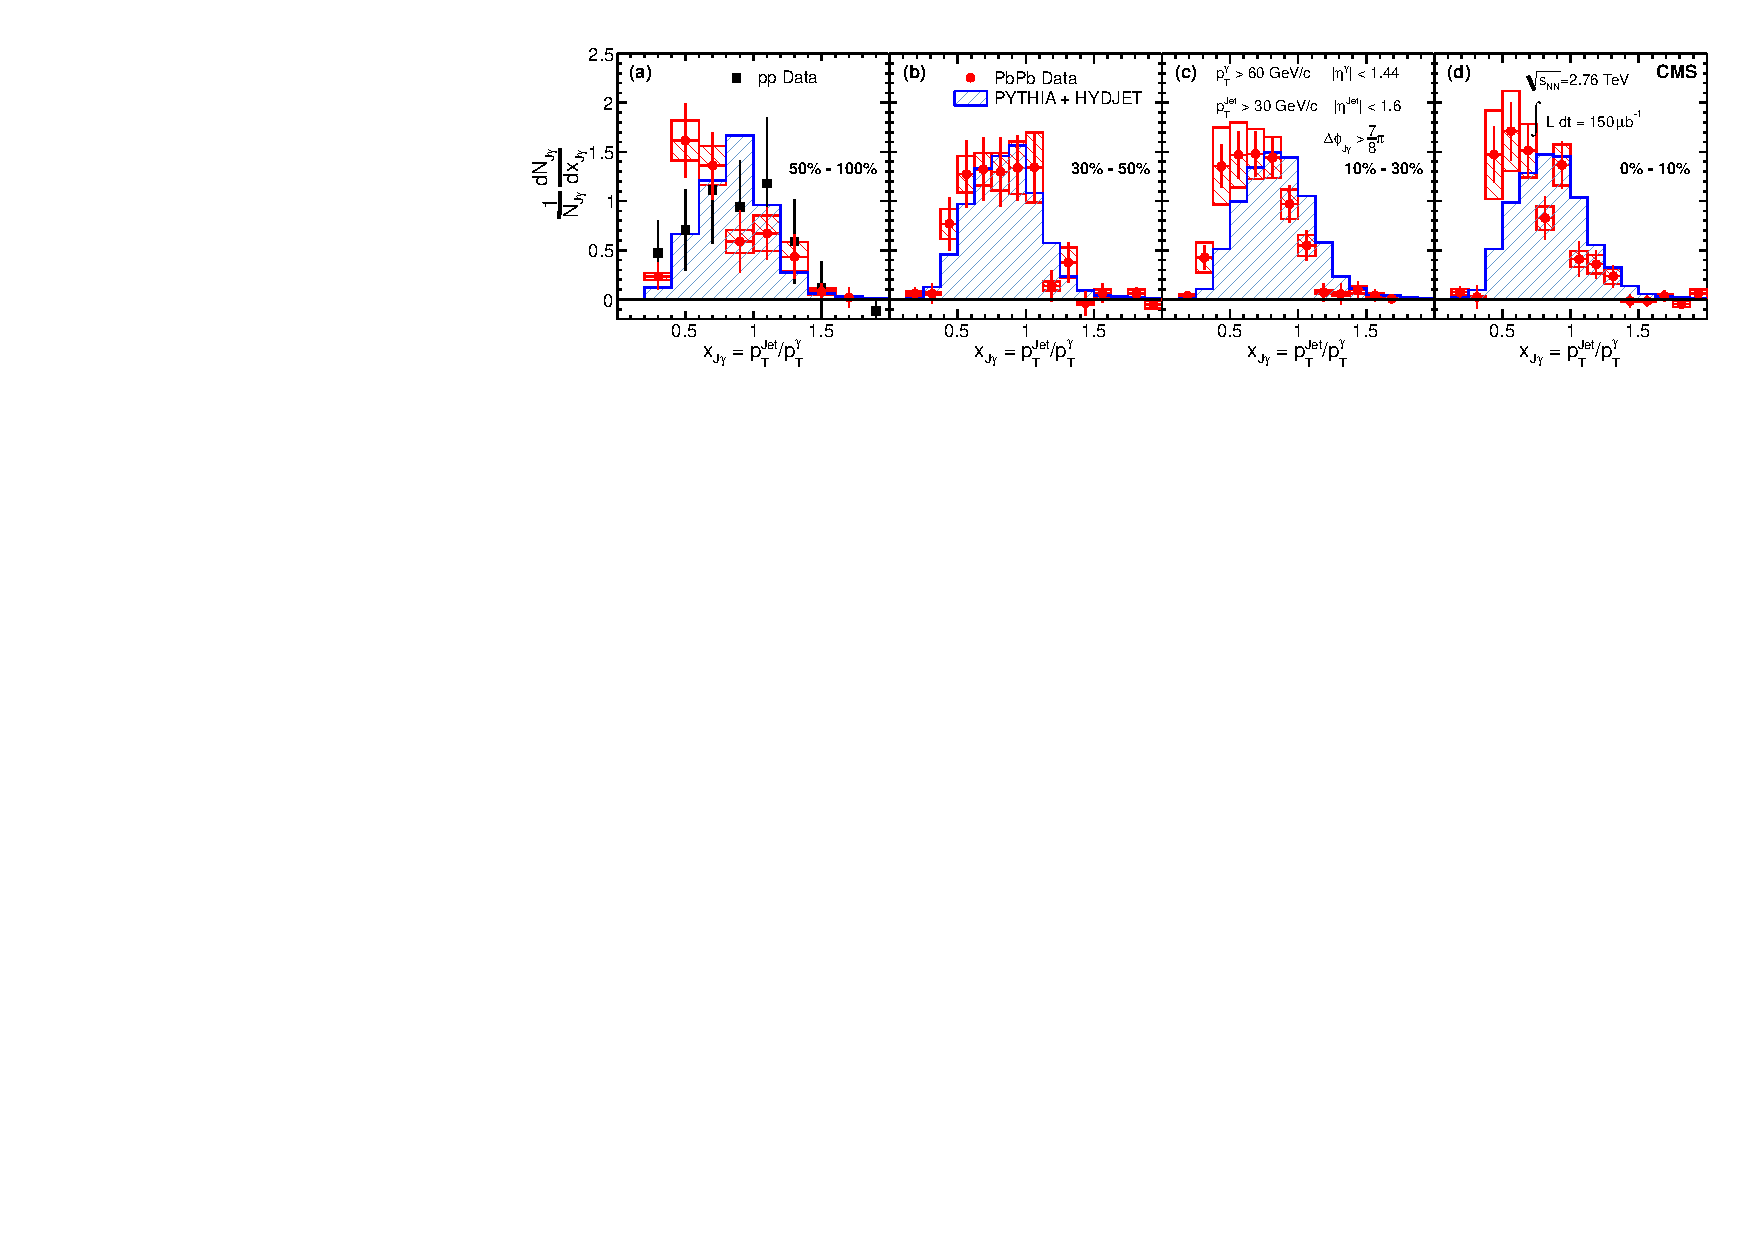
\includegraphics[width=0.98\mboxwidth]{jetfigures/Photonv7_Paper_InclPtRatio_all_cent4_G60J30_subDPhi1SS1_Isol0_Norm1log1.pdf}
\caption[]{\label{fig:InclPtRatio_qcdPhoRef_pp2760-xJ30G60} Ratio of \pt{} between the
  photon ($\pt^{\gamma} > 60$\GeVc) and jet ($\pt^{\mbox{Jet}} > 30$\GeVc, $\dphijg > \frac{7}{8}\pi$)
  after subtracting background. The area of each distribution is normalised to unity. All panels show
\PbPb\ data (filled circles) compared to \pp\ data at
  2.76\TeV (filled squares), and to the \PYTHYD{} MC simulation
  (shaded histogram) in bins of increasing centrality left to right. The error bars
  on the points represent the statistical uncertainty.
  See mbox for an explanation of the open and shaded red systematic
  uncertainty boxes.
}
\label{fig:GR:CMS_xjg}
\end{center}
\end{figure}

It is important to keep in mind that the average energy loss of the selected \photonjet\ pairs does not constitute the full picture.
There are genuine \photonjet\ events which do not contribute to the $\langle\xjg\rangle$ distribution
because the associated  jet falls below the $\ptj > 30\GeVc$ threshold.
To quantify this effect, Fig.~\ref{fig:resultsummarybc}(b) shows $\rjg$, the fraction of isolated photons that have an associated jet passing the analysis selection.
The value of $\rjg$ is found to
decrease, from $\rjg = 0.685\pm 0.008\mbox{(stat.)}$--$0.698\pm 0.006\mbox{(stat.)}$ for the \PYTHYD{} reference,
as well as \pp{} and peripheral \PbPb{} data, to the significantly
lower $\rjg = 0.49\pm 0.03\mbox{(stat.)}\pm 0.02\mbox{(syst.)}$--$0.54\pm 0.05\mbox{(stat.)}\pm 0.02\mbox{(syst.)}$ for
the three PbPb bins
above 50\% centrality.

The first study of isolated-photon+jet correlations in
  $\PbPb$ collisions at $\sqrt{s_{NN}} = 2.76\TeV$ has been performed as a function of collision centrality using
a dataset corresponding to an integrated luminosity of 150\mubinv. Isolated
photons with $\ptg > 60$\GeVc were correlated with jets with $\ptj > 30$\GeVc to
determine the width of the angular
correlation function, \sjg, the jet/photon transverse momentum ratio, $\xjg = \ptj/\ptg$, and
the fraction of photons with an associated jet, \rjg.
The \PbPb{} data were compared to both \pp{} data and a \PYTHYD{} MC reference which included the effect of the underlying \PbPb event
but no parton energy loss.
No angular broadening was observed beyond that seen in the pp data and MC reference at all centralities.
The average transverse momentum ratio for the most central events was found to be
$\avexjg_{0-10\%} = 0.73 \pm 0.02 \mbox{(stat.)} \pm 0.04 \mbox{(syst.)}$.
This is lower than the value of 0.86 seen in the pp data and predicted by \PYTHYD{} at the same centrality.
In addition to the shift in
momentum balance, it was found that, in central \PbPb\ data, only
a fraction equal to $\rjg = 0.49 \pm 0.03 \mbox{ (stat.)} \pm 0.02 \mbox{ (syst.)}$ of photons are matched with an
associated jet at $\dphijg > \frac{7}{8} \pi$, compared to a value of 0.69 seen
in \PYTHYD{} simulation. Due to the hot and dense medium created in central \PbPb\ collisions, the energy loss of the associated parton causes the corresponding reconstructed jet to fall
below the $\ptj > 30$\GeVc threshold for an additional 20\% of the selected photons.
